\documentclass{beamer}

\pdfmapfile{+sansmathaccent.map}


\mode<presentation>
{
  \usetheme{Warsaw} % or try Darmstadt, Madrid, Warsaw, Rochester, CambridgeUS, ...
  \usecolortheme{crane} % or try seahorse, beaver, crane, wolverine, ...
  \usefonttheme{serif}  % or try serif, structurebold, ...
  \setbeamertemplate{navigation symbols}{}
  \setbeamertemplate{caption}[numbered]
} 


%%%%%%%%%%%%%%%%%%%%%%%%%%%%
% itemize settings

\definecolor{myhotpink}{RGB}{255, 80, 200}
\definecolor{mywarmpink}{RGB}{255, 60, 160}
\definecolor{mylightpink}{RGB}{255, 80, 200}
\definecolor{mypink}{RGB}{255, 30, 80}
\definecolor{mydarkpink}{RGB}{155, 25, 60}
\definecolor{myblue}{RGB}{240, 240, 255}
\definecolor{mydarkblue}{RGB}{60, 160, 255}
\definecolor{mygreen}{RGB}{0, 200, 0}
\definecolor{mygreen2}{RGB}{245, 255, 230}
\definecolor{mygray}{gray}{0.8}


\definecolor{mydarkcolor}{RGB}{60, 25, 155}
\definecolor{mylightcolor}{RGB}{130, 180, 250}

\setbeamertemplate{itemize items}[default]

\setbeamertemplate{itemize item}{\color{mywarmpink}$\blacksquare$}
\setbeamertemplate{itemize subitem}{\color{mydarkblue}$\blacktriangleright$}
\setbeamertemplate{itemize subsubitem}{\color{mygray}$\blacksquare$}



\setbeamercolor{palette quaternary}{fg=white,bg=mydarkcolor}
\setbeamercolor{titlelike}{parent=palette quaternary}

\setbeamercolor{palette quaternary2}{fg=black,bg=mylightcolor}
\setbeamercolor{frametitle}{parent=palette quaternary2}



\setbeamerfont{frametitle}{size=\Large,series=\scshape}
\setbeamerfont{framesubtitle}{size=\normalsize,series=\upshape}


%%%%%%%%%%%%%%%%%%%%%%%%%%%%
% block settings

\setbeamercolor{block title}{bg=red!50,fg=black}

\setbeamercolor*{block title example}{bg=mygreen!40!white,fg=black}

\setbeamercolor*{block body example}{fg= black,
bg= mygreen2}


%%%%%%%%%%%%%%%%%%%%%%%%%%%%
% URL settings
\hypersetup{
    colorlinks=false,
    linkcolor=blue,
    filecolor=blue,      
    urlcolor=blue,
}

%%%%%%%%%%%%%%%%%%%%%%%%%%

\renewcommand{\familydefault}{\rmdefault}

\usepackage{amsmath}
\usepackage{mathtools}

\usepackage{subcaption}


\newcommand{\mydate}{Spring 2022}
\newcommand{\mygit}{\textcolor{blue}{\href{https://github.com/SergeiSa/Computational-Intelligence-Slides-Spring-2022}{github.com/SergeiSa/Computational-Intelligence-Slides-Spring-2022}}}

\newcommand{\bo}[1] {\mathbf{#1}}
\newcommand{\R} {\mathbb{R}}
\DeclareMathOperator*{\argmin}{arg\,min}


%%%%%%%%%%%%%%%%%%%%%%%%%%%%
% code settings

\usepackage{listings}
\usepackage{color}
% \definecolor{mygreen}{rgb}{0,0.6,0}
% \definecolor{mygray}{rgb}{0.5,0.5,0.5}
\definecolor{mymauve}{rgb}{0.58,0,0.82}
\lstset{ 
  backgroundcolor=\color{white},   % choose the background color; you must add \usepackage{color} or \usepackage{xcolor}; should come as last argument
  basicstyle=\footnotesize,        % the size of the fonts that are used for the code
  breakatwhitespace=false,         % sets if automatic breaks should only happen at whitespace
  breaklines=true,                 % sets automatic line breaking
  captionpos=b,                    % sets the caption-position to bottom
  commentstyle=\color{mygreen},    % comment style
  deletekeywords={...},            % if you want to delete keywords from the given language
  escapeinside={\%*}{*)},          % if you want to add LaTeX within your code
  extendedchars=true,              % lets you use non-ASCII characters; for 8-bits encodings only, does not work with UTF-8
  firstnumber=0000,                % start line enumeration with line 0000
  frame=single,	                   % adds a frame around the code
  keepspaces=true,                 % keeps spaces in text, useful for keeping indentation of code (possibly needs columns=flexible)
  keywordstyle=\color{blue},       % keyword style
  language=Octave,                 % the language of the code
  morekeywords={*,...},            % if you want to add more keywords to the set
  numbers=left,                    % where to put the line-numbers; possible values are (none, left, right)
  numbersep=5pt,                   % how far the line-numbers are from the code
  numberstyle=\tiny\color{mygray}, % the style that is used for the line-numbers
  rulecolor=\color{black},         % if not set, the frame-color may be changed on line-breaks within not-black text (e.g. comments (green here))
  showspaces=false,                % show spaces everywhere adding particular underscores; it overrides 'showstringspaces'
  showstringspaces=false,          % underline spaces within strings only
  showtabs=false,                  % show tabs within strings adding particular underscores
  stepnumber=2,                    % the step between two line-numbers. If it's 1, each line will be numbered
  stringstyle=\color{mymauve},     % string literal style
  tabsize=2,	                   % sets default tabsize to 2 spaces
  title=\lstname                   % show the filename of files included with \lstinputlisting; also try caption instead of title
}

%%%%%%%%%%%%%%%%%%%%%%%%%%%%
% tikz settings

\usepackage{tikz}
\tikzset{every picture/.style={line width=0.75pt}}

%%%%%%%%%%%%%%%%%%%%%%%%%%%%

\usepackage{qrcode}



\title{Barrier functions}
\subtitle{Computational Intelligence, Lecture 11}
\author{by Sergei Savin}
\centering
\date{\mydate}



\begin{document}
\maketitle


\begin{frame}{Content}

\begin{itemize}
\item Linear inequalities
\item Barrier functions
\item Barrier functions for QPs
\item Analytic center of linear inequalities
\item Homework
\end{itemize}

\end{frame}



\begin{frame}{Linear inequalities}
% \framesubtitle{General form}
\begin{flushleft}

Consider linear inequality constraints:

\begin{equation}
    \bo{A}\bo{x} \leq \bo{b}
\end{equation}

Remember that we can rewrite it as:

\begin{equation}
    \bo{a}_i^\top \bo{x} \leq b_i
\end{equation}
\begin{equation}
\label{eq:linear_constraints}
    \bo{a}_i^\top \bo{x} - b_i \leq 0
\end{equation}

Instead of \emph{hard constraints} in \eqref{eq:linear_constraints} we can turn these into a cost function component:

\begin{equation}
    J = -\sum\limits_{i = 1}^n \text{log} (b_i - \bo{a}_i^\top \bo{x})
\end{equation}

Which is called a \emph{barrier function}.
 
\end{flushleft}
\end{frame}




\begin{frame}{Barrier functions}
% \framesubtitle{General form}
\begin{flushleft}

Let us consider barrier functions $J = -\sum\limits_{i = 1}^n \text{log} (b_i - \bo{a}_i^\top \bo{x})$:

\begin{itemize}
    \item It removes the constraint, but modifies the cost.
    \item When $b_i - \bo{a}_i^\top \bo{x}$ is a very small positive number, $\text{log} (b_i - \bo{a}_i^\top \bo{x})$ is a very big negative number, hence the minus sign in front.
    \item Barrier function does not behave well outside of the domain, when $b_i - \bo{a}_i^\top \bo{x} < 0$.
\end{itemize}
 
\end{flushleft}
\end{frame}




\begin{frame}{Barrier functions for QPs}
% \framesubtitle{General form}
\begin{flushleft}

Hence the following QP:

\begin{equation}
\begin{aligned}
& \underset{\bo{x}}{\text{minimize}}
& & \bo{x}^\top \bo{H} \bo{x} + \bo{f}^\top \bo{x}, \\
& \text{subject to}
& & \begin{cases}
    \bo{A}\bo{x} \leq \bo{b}, \\
    \bo{C}(\bo{x}) = \bo{d}.
    \end{cases}
\end{aligned}
\end{equation}
 
...can be approximated as:

\begin{equation}
\begin{aligned}
& \underset{\bo{x}}{\text{minimize}}
& & \bo{x}^\top \bo{H} \bo{x} + \bo{f}^\top \bo{x} - \sum\limits_{i = 1}^n \text{log} (b_i - \bo{a}_i^\top \bo{x}), \\
& \text{subject to}
& & \bo{C}(\bo{x}) = \bo{d}
\end{aligned}
\end{equation}
 
\end{flushleft}
\end{frame}




\begin{frame}{Analytic center of linear inequalities}
% \framesubtitle{General form}
\begin{flushleft}

We can define \emph{analytic center of linear inequalities} as a minimum of the function $J = -\sum\limits_{i = 1}^n \text{log} (b_i - \bo{a}_i^\top \bo{x})$. And that can be solved as a convex optimization:

\begin{align*}
    \bo{x}_a = \underset{\bo{x}}{\text{argmin}} & \ \  -\sum\limits_{i = 1}^n \text{log} (b_i - \bo{a}_i^\top \bo{x})
\end{align*}

At the analytic center of linear inequalities the shape of contour lines can be analysed as a local quadratic approximation of the function $J$:

\begin{equation}
    \mathcal{C} = \{ \bo{x}: \ (\bo{x} - \bo{x}_a)^\top \frac{\partial^2 J}{\partial \bo{x}^2} (\bo{x} - \bo{x}_a) = \epsilon \}
\end{equation}

where $\epsilon$ is a small number.
  
\end{flushleft}
\end{frame}



\begin{frame}{Illustration of a barrier functions}
% \framesubtitle{Parameter estimation}
\begin{flushleft}

\begin{figure}
    \centering
    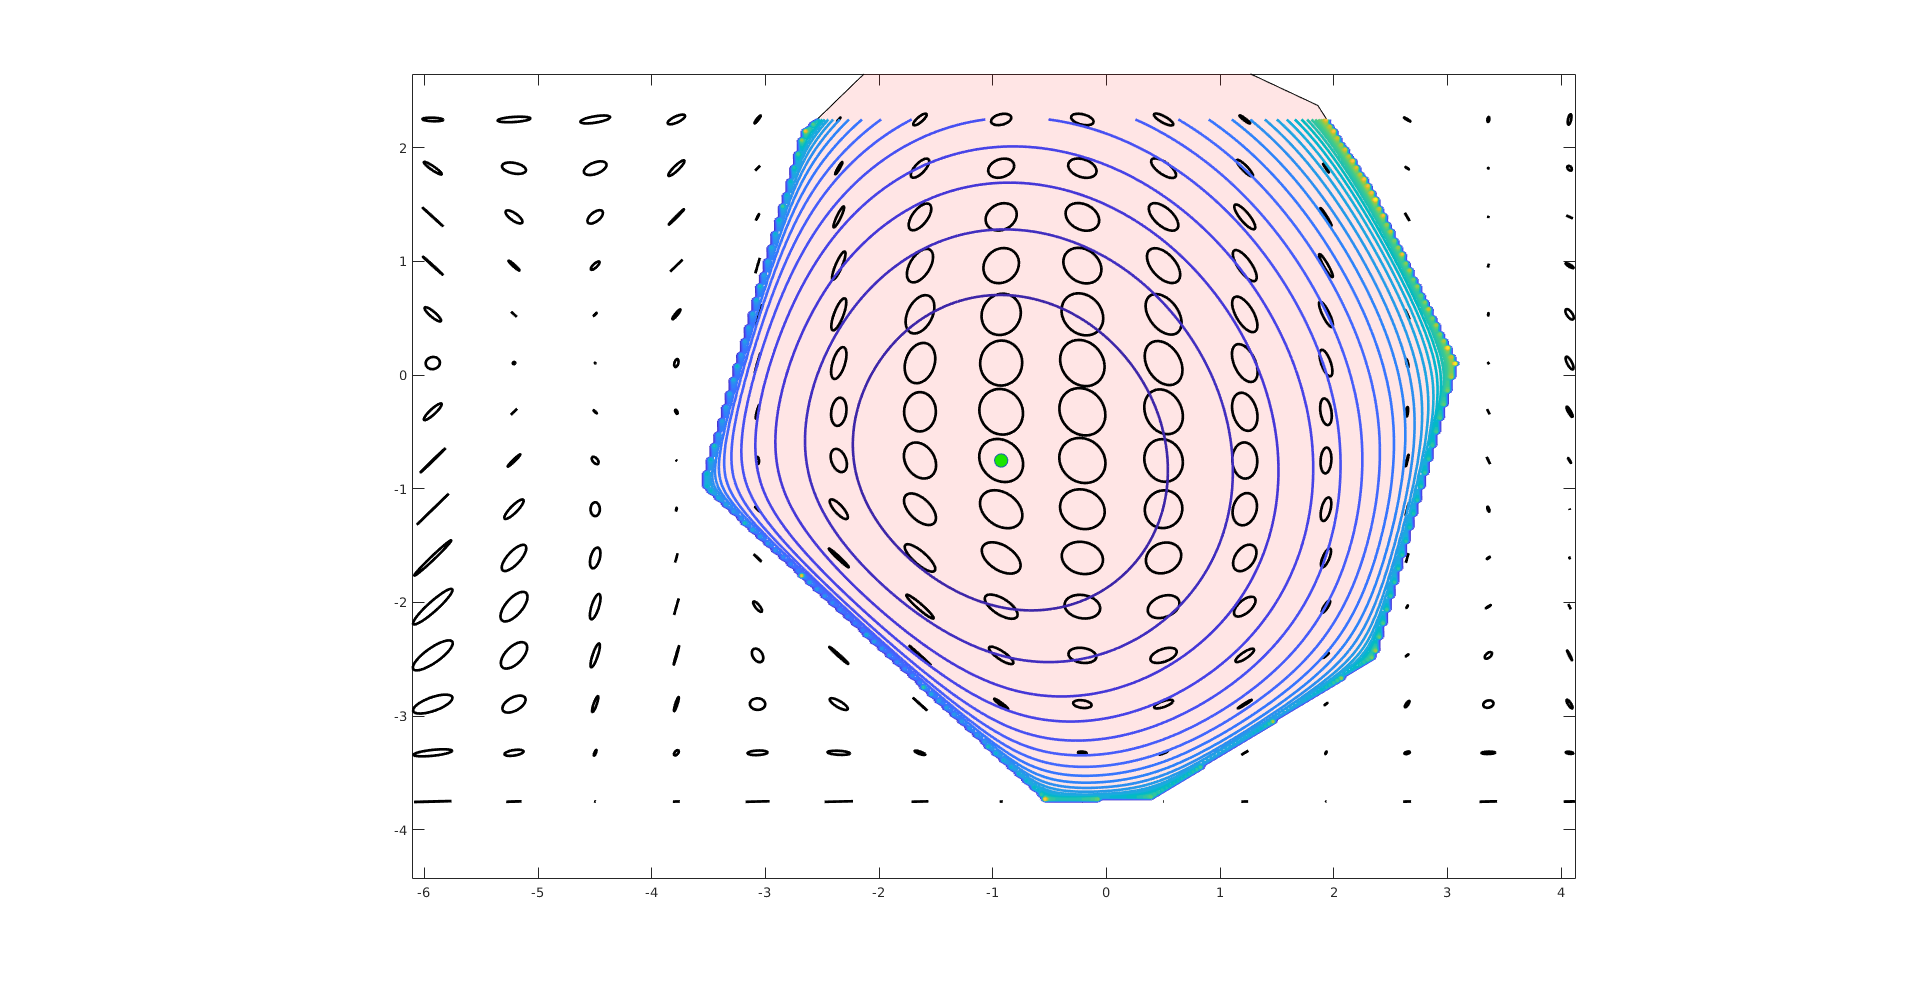
\includegraphics[width=\linewidth]{LogBarrier2.png}
    \caption{Barrier functions}
    \label{fig:BarrierFunctions}
\end{figure}

Pink is the domain. The ellipsoids represent the shape of the hessian $\frac{\partial^2 J}{\partial \bo{x}^2}$ at different points on the domain. Green dot is $\bo{x}_a$.

\end{flushleft}
\end{frame}




\begin{frame}{Lagrangian}
	% \framesubtitle{General form}
	\begin{flushleft}
		
		Consider an optimization problem:
		
		\begin{equation}
			\begin{aligned}
				& \underset{\bo{x}}{\text{minimize}}
				& & f_0(\bo{x}), \\
				& \text{subject to}
				& & \begin{cases}
					f_i(\bo{x}) \leq 0, \\
					h_j(\bo{x}) = 0.
				\end{cases}
			\end{aligned}
		\end{equation}
		
		It's \emph{Lagrangian} is given as:
		
		\begin{equation}
			L(\bo{x}, \lambda_i, \nu_j) = 
			f_0(\bo{x}) + 
			\sum\limits_i \lambda_i f_i(\bo{x}) +
			\sum\limits_j \nu_j h_j(\bo{x})
		\end{equation}
	%
	where $\lambda_i$ and $\nu_j$ are Lagrange multipliers; they are sometimes called \emph{dual variables}.
		
	\end{flushleft}
\end{frame}



\begin{frame}{Lagrange dual function}
	% \framesubtitle{General form}
	\begin{flushleft}
		
	Given \emph{Lagrangian} $L(\bo{x}, \lambda_i, \nu_j) = 
	f_0(\bo{x}) + 
	\sum\limits_i \lambda_i f_i(\bo{x}) +
	\sum\limits_j \nu_j h_j(\bo{x})$, the associated 
	 \emph{Lagrange dual function} is given as:
		
		\begin{equation}
			g(\lambda_i, \nu_j)  = \underset{\bo{x}}{\text{inf}}
			\ L(\bo{x}, \lambda_i, \nu_j).
		\end{equation}
		
		Lagrange dual function is always concave. If $p^*$ is the optimal value of the cost function of the original problem, then $g(\lambda_i, \nu_j)$ gives as a \emph{lower bound} on its possible values. In fact, substituting any $\nu_j$ and $\lambda_i > 0$ gives us a valid lower bound on the cost. Maximum of $g(\lambda_i, \nu_j)$ over the domain given by $\lambda_i > 0$ provides us optimal (largest) lower bound of the problem, denoted as $g^*$. 
		
	\end{flushleft}
\end{frame}



\begin{frame}{Duality gap, strong and weak duality}
	% \framesubtitle{General form}
	\begin{flushleft}
		
		If $p^*$ is the optimal value of the cost function of the original problem and $g^*$ is the optimal lower bound of the problem, then $p^* - g^*$ is called optimal \emph{duality gap}.
		
		\bigskip
		
		If optimal duality gap is zero, the problem is said to have \emph{strong duality}. If optimal duality gap greater than zero, the problem is said to have \emph{weak duality}.
		
	\end{flushleft}
\end{frame}



\begin{frame}{Lagrange dual function for a QP, 1}
	% \framesubtitle{General form}
	\begin{flushleft}
		
		Consider the following QP:
		
		\begin{equation}
			\begin{aligned}
				& \underset{\bo{x}}{\text{minimize}}
				& & \bo{x}^\top \bo{H} \bo{x}, \\
				& \text{subject to}
				& & \bo{A}\bo{x} \leq \bo{b}.
			\end{aligned}
		\end{equation}
		%
		Its Lagrangian is:
		%
		\begin{equation}
			L(\bo{x}, \lambda) = \bo{x}^\top \bo{H} \bo{x} + \lambda^\top (\bo{A}\bo{x} - \bo{b})
		\end{equation}
		
		In order to minimize the Lagrangian with respect to $\bo{x}$ we find the gradient and set it to zero:
		%
		\begin{equation}
			\frac{L(\bo{x}, \lambda)}{\bo{x}} = 2\bo{x}^\top \bo{H} + \lambda^\top \bo{A} = 0
		\end{equation}
		
		With that we can compute $\bo{x}$ as a function of $\lambda$:
		%
		\begin{equation}
			\bo{x} = -0.5\bo{H}^{-1}\bo{A}^\top \lambda
		\end{equation}
		
	\end{flushleft}
\end{frame}



\begin{frame}{Lagrange dual function for a QP, 2}
	% \framesubtitle{General form}
	\begin{flushleft}
		
		Knowing that $\bo{x} = -0.5\bo{H}^{-1}\bo{A}^\top \lambda$ we can compute $g(\lambda)$ by substituting the $\bo{x}$ we found into the Lagrangian:
		%
		\begin{equation}
			g(\lambda) = \frac{1}{4} \lambda^\top \bo{A}\bo{H}^{-1}\bo{H}\bo{H}^{-1}\bo{A}^\top\lambda - \frac{1}{2} \lambda^\top \bo{A}\bo{H}^{-1}\bo{A}^\top \lambda - \lambda^\top\bo{b}
		\end{equation}
	%
	\begin{equation}
		g(\lambda) = -\frac{1}{4} \lambda^\top \bo{A}\bo{H}^{-1}\bo{A}^\top\lambda - \lambda^\top\bo{b}
	\end{equation}
		
		In order to find the optimal lower bound we solve the following problem:
		%
		\begin{equation}
			\begin{aligned}
				& \underset{\lambda}{\text{maximize}}
				& & -\frac{1}{4} \lambda^\top \bo{A}\bo{H}^{-1}\bo{A}^\top\lambda - \lambda^\top\bo{b}, \\
				& \text{subject to}
				& & \lambda \geq 0.
			\end{aligned}
		\end{equation}
		
		Note that optimal values of $\lambda$ determine local sensitivity of the system with respect to small perturbations of constraints.
		
	\end{flushleft}
\end{frame}




\begin{frame}{Example, sensitivity}
	% \framesubtitle{General form}
	\begin{flushleft}
		
	
		Consider minimizing $(\bo{x} - \bo{c})^\top (\bo{x} - \bo{c})$ when the domain is the second quadrant: $x_1 \geq 0$ and $x_2 \leq 0$. Find sensitivity of the problem as a function of $\bo{c}$.
	%
		\begin{equation}
			\begin{aligned}
				& \underset{\bo{x}}{\text{minimize}}
				& & (\bo{x} - \bo{c})^\top (\bo{x} - \bo{c}), \\
				& \text{subject to}
				& & \bo{A}\bo{x} \leq 0.
			\end{aligned}
		\end{equation}
	%
	where $\bo{A} = \begin{bmatrix}
		-1 & 0 \\ 0 & 1
	\end{bmatrix}$.
		
		The dual Lagrange function is:
		
		\begin{equation}
			g(\lambda) = -\frac{1}{4} \lambda^\top \bo{A}\bo{A}^\top\lambda + \lambda^\top \bo{A}\bo{c}
		\end{equation}
		
		
	\end{flushleft}
\end{frame}



\begin{frame}{Example, Illustration of the sensitivity}
	% \framesubtitle{Parameter estimation}
	\begin{flushleft}
		
		\begin{figure}
			\centering
			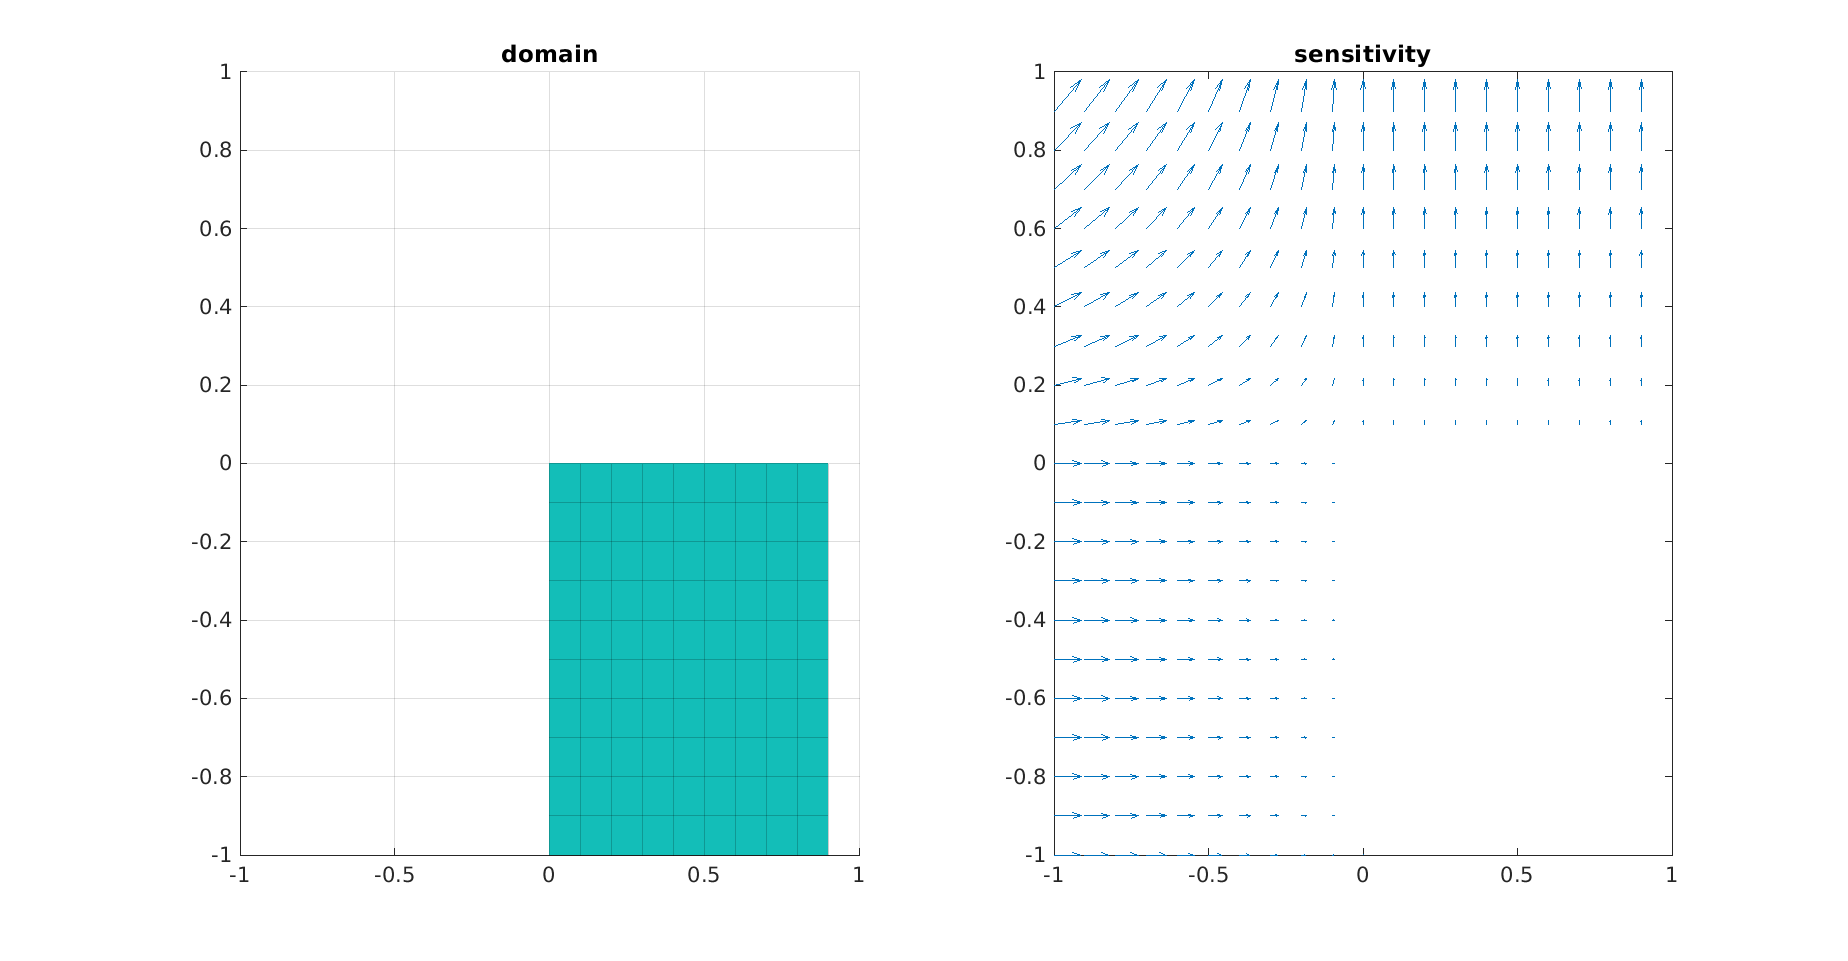
\includegraphics[width=\linewidth]{sensitivity.png}
			\caption{Sensitivity}
			\label{fig:Sensitivity}
		\end{figure}
		
		Turquoise on the left is the domain. The arrows on the right show the values of $\lambda$.
		
	\end{flushleft}
\end{frame}





\begin{frame}{Homework}
% \framesubtitle{Parameter estimation}
\begin{flushleft}

Visualize contours of a quadratic program of your choice. Compute its optimal lower bound and duality gap.

\end{flushleft}
\end{frame}





\begin{frame}
	\centerline{Lecture slides are available via Moodle.}
	\bigskip
	\centerline{You can help improve these slides at:}
	\centerline{
		\mygit
	}
	\bigskip
	
	\textcolor{black}{\qrcode[height=1.5in]{https://github.com/SergeiSa/Computational-Intelligence-Slides-Spring-2022}}
	\bigskip
	
	
	\centerline{Check Moodle for additional links, videos, textbook suggestions.}
\end{frame}



\end{document}
